\section*{Results}\label{s:results}

\subsection*{Citations and full size figures with legends underneath}

Text is added like this
This is a reference to a published paper \citep{watson_molecular_1953}.
We can cite other things too \citep{tipton_complexities_2019,zheng_genome_2011,alberts_molecular_2002}

This is a new paragraph.
New sentences on a new line.
New sentences on a new line.

% this is how to add a comment
This is a new result.
% this is how to add a figure with the name cells.
As you can see (Figure \ref{fig:cells}).

% full size figure is figure*
\begin{figure*}
\centering
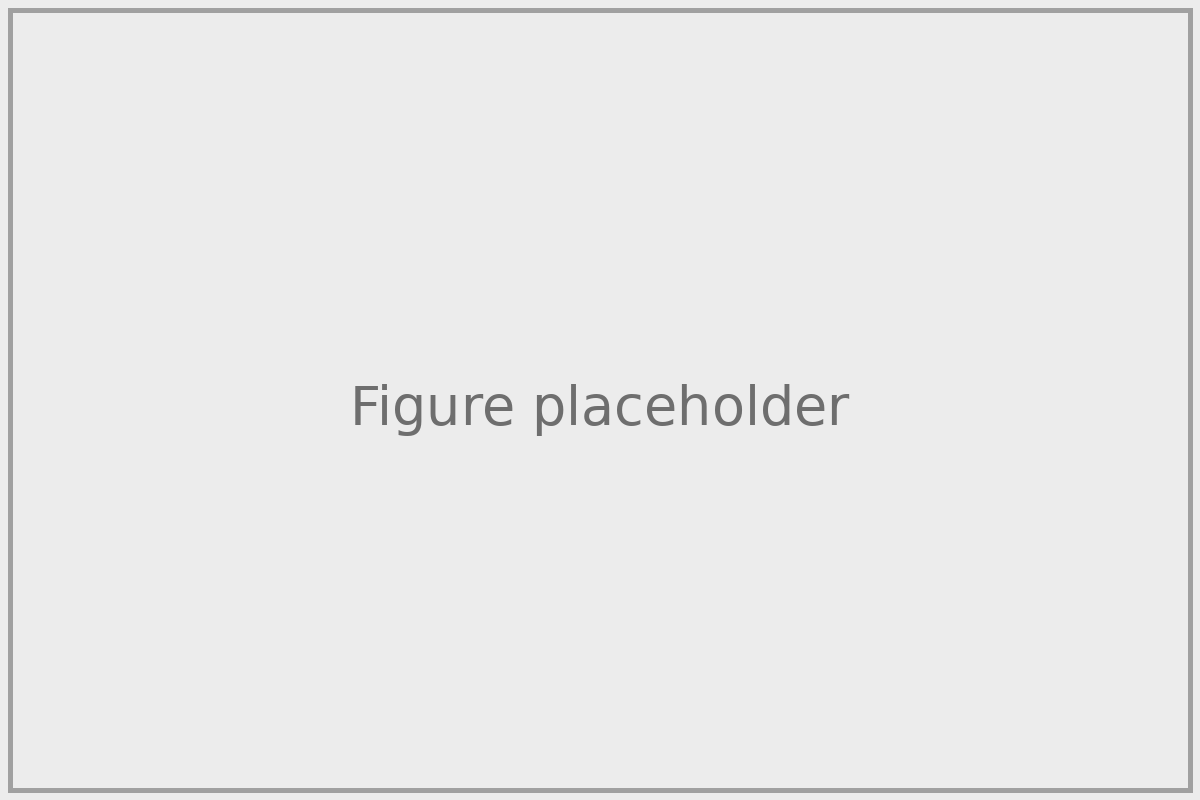
\includegraphics[width=0.75\linewidth]{assets/placeholder.png}
\caption{\textbf{These are cells.}\\
(\textbf{A}) This is a regular figure with a legend as a caption underneath. Inset: 3X zoom. Scale bar, \SI{10}{\micro\meter}.}
\label{fig:cells}
\end{figure*}

It is possible to add a one-column Figure like this (Figure \ref{fig:nucleus}).
To add Supplementary Figures you can do either of these things and have them at the end of the end of the paper (Supplementary Figure \ref{suppfig:endosome}).
Or like this (Supplementary Figure \ref{videosupp:lysosome}).

\lipsum[10]

\subsection*{Subsections are written like this}

\lipsum[11]

% one-column size figure is figure
\begin{figure}
\centering
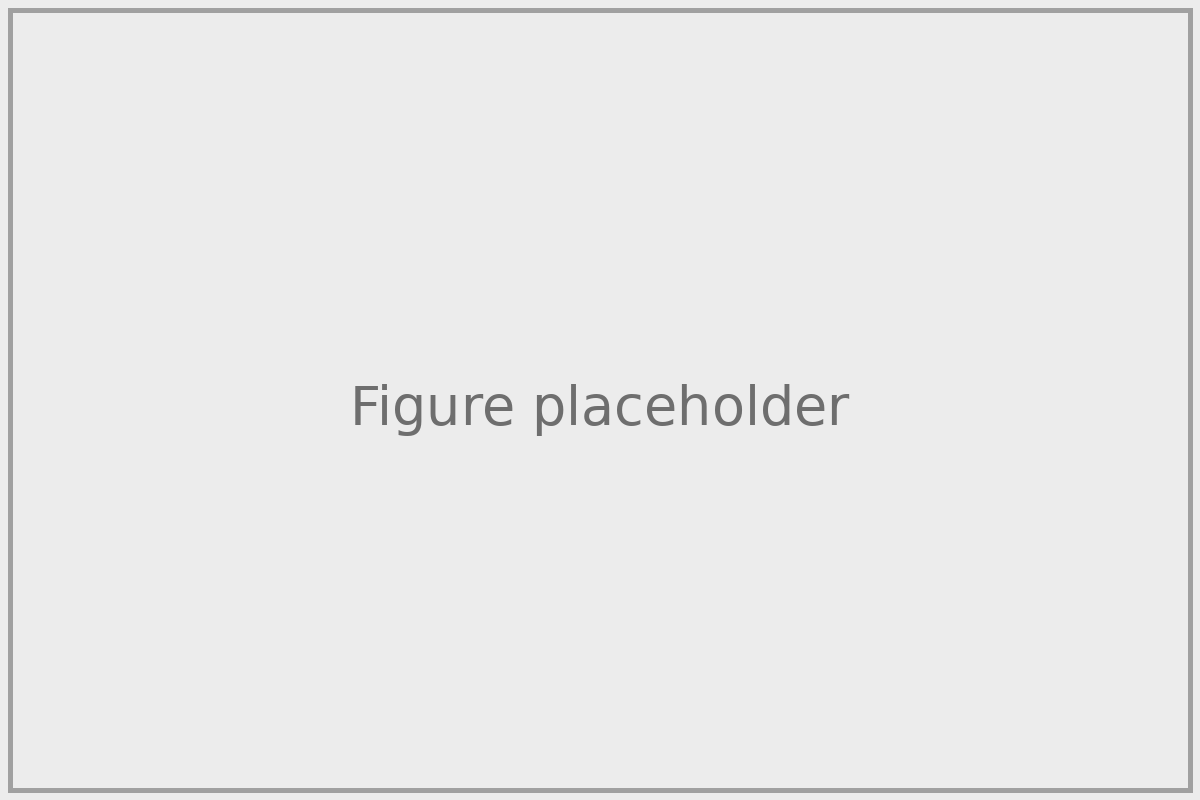
\includegraphics[width=0.75\linewidth]{assets/placeholder.png}
\caption{\textbf{This is a nucleus.}\\
(\textbf{A}) This is a one-column figure with a legend as a caption underneath.}
\label{fig:nucleus}
\end{figure}

\lipsum[12]

\subsection*{Another subsection}

\lipsum[13-14]

\subsection*{Another subsection}

\lipsum[13-14]

\subsection*{Another subsection}

\lipsum[13-14]
